\begin{frame}
\begin{itemize}
\item Sample statistic - How salty the spoonful is
\item Population parameter - How salty the whole pot is
\item We often estimate the population parameter from the sample statistic.
\end{itemize}
\pause
Gwen has 2000 goats. She randomly selects 30 of her goats to measure their weights and finds an average weight of 80 pounds.
\dq{What is the sample?} 
\pause \soln{The 30 goats.}
\dq{What is the population?}
\pause \soln{The 2000 goats.}
\dq{What is the sample statistic?}
\pause \soln{The 30 goats' average weight is {\bf 80 pounds}.}
\dq{What is the population parameter?}
\pause \soln{The unknown average weight of all 2000 goats.}
\end{frame}

%%%%%%%%%%%%%%%%%%%%%%%%%%%%%%%%%%%%%



%%%%%%%%%%%%%%%%%%%%%%%%%%%%%%%%%%%%

\begin{frame}
\frametitle{Observational studies vs. experiments}
\pause
\begin{itemize}
\item In observational studies, data are collected only by monitoring what occurs. Observational studies show associations (not causal relationships).
\pause
\item Experiments require the primary explanatory variable in a study be (randomly) assigned for each subject by the researchers. Experiments can show causal relationships.
\end{itemize}


\pause
\begin{center} \footnotesize
\begin{tabular}{|c|c|c|} \hline
                      & \bf Experiment &  \bf Observational study \\ \hline
\bf representative sample & Best!      & No causality \\\hline
\bf biased sample         & Can't generalize to population & useless \\ \hline
\end{tabular}
\end{center}
\end{frame}


\begin{frame}
\frametitle{Causality}
Experiments can show {\bf causality}. For example, experiments can show alcohol impairs driving ability. How would you run this experiment?

\pause
If we are considering a causal relationship, we are suggesting that by changing the {\bf explanatory variable}, we can expect changes in the {\bf response variable}.
\pause
\dq{With alcohol and driving ability, determine the explanatory variable.} \pause
\soln{The explanatory variable would be whether the driver was given alcohol.} \pause
\dq{With alcohol and driving ability, determine the response variable.} \pause
\soln{The response variable would be performance on some driving task(s).}


\end{frame}


\begin{frame}
Suppose an observational study tracked sunscreen use and skin cancer, and it was found that the more sunscreen someone used, the more likely the person was to have skin cancer. Does this mean sunscreen causes skin cancer?
\pause
\dq{What is the suggested explanatory variable?}
\pause
\soln{Amount of sunscreen used.}
\pause

\vspace{10pt}
\dq{What is the suggested response variable?}
\pause
\soln{Likelihood of skin cancer.}
\pause

\vspace{10pt}
\dq{What is a possible confounding (lurking) variable?}
\pause
\soln{Whether the person lives in a sunny area or whether the person is pale}

\end{frame}




%\section{Observational studies and sampling strategies}

%%%%%%%%%%%%%%%%%%%%%%%%%%%%%%%%%%

\subsection{Confounding}

%%%%%%%%%%%%%%%%%%%%%%%%%%%%%%%%%%%%

\begin{frame}
\frametitle{Confounding variables}
A {\bf confounding variable} is a third variable that may cause two other variables to have an association.
\pause
\begin{center}
\includegraphics[scale=0.6]{1-4_obs_studies_sampling/figures/sun/sunCausesCancer}
\end{center}
\pause
Sun exposure is a confounding variable that may explain why more suncreen is associated with more cancer.
\end{frame}

\begin{frame}
Imagine a study finds a positive association between amount of ice cream a community eats and the rate of drowning in that community.

\pause
Do you think ice cream causes drowning?

\pause
Do you think drownings cause ice cream?
\pause

\vspace{10pt}
\dq{What could be a confounding variable?}
\soln{Maybe hot temperatures cause more ice cream and more drowning.}
\end{frame}


\begin{frame}
\frametitle{Identify possible confounding variables}
\dq{Sleeping with one's shoes on is strongly correlated with waking up with a headache. \\Therefore, sleeping with one's shoes on causes headache.}\pause
\soln{Both may be caused by drunkiness}

\pause
\dq{Young children who sleep with the light on are much more likely to develop myopia in later life.\\ 
    Therefore, sleeping with the light on causes myopia.}\pause
\soln{Myopic parents are more likely to leave the light on in child's room.}\pause

\dq{People who drink Gatorade are more likely to develop knee injuries.\\
    Therefore, drinking Gatorade causes knee injuries.}\pause
\soln{Whether someone is an athlete causes higher chance of both drinking Gatorade and getting knee injuries.}\pause
\end{frame}



%%%%\begin{frame}
%%%%\frametitle{}

%%%%\begin{center}
%%%%\includegraphics[width=0.80\textwidth]{1-4_obs_studies_sampling/figures/breakfast/breakfast1}
%%%%\end{center}

%%%%{\tiny \webURL{http://www.peertrainer.com/LoungeCommunityThread.aspx?ForumID=1\&ThreadID=3118}}

%%%%\end{frame}

%%%%%%%%%%%%%%%%%%%%%%%%%%%%%%%%%%%%%%%%

%%%%\begin{frame}
%%%%\frametitle{}

%%%%\dq{What type of study is this, observational study or an experiment?
%%%%{\footnotesize \textit{``Girls who regularly ate breakfast, particularly one that includes cereal, were slimmer than those who skipped the morning meal, according to a study that tracked nearly 2,400 girls for 10 years. [...] As part of the survey, the girls were asked once a year what they had eaten during the previous three days."}}
%%%%}

%%%%\soln{\onslide<2->{This is an \hl{observational study} since the researchers merely observed the behavior of the girls (subjects) as opposed to imposing treatments on them.}}

%%%%\dq{What is the conclusion of the study?}

%%%%\soln{\onslide<3->{There is an \hl{association} between girls eating breakfast and being slimmer.}}

%%%%\dq{Who sponsored the study?}

%%%%\soln{\onslide<4->{General Mills.}}

%%%%\end{frame}

%%%%%%%%%%%%%%%%%%%%%%%%%%%%%%%%%%%%%%%%

%%%%\begin{frame}[shrink]
%%%%\frametitle{3 possible explanations}

%%%%\pause

%%%%\begin{enumerate}

%%%%\item Eating breakfast causes girls to be thinner.
%%%%\begin{center}
%%%%\includegraphics[width=0.5\textwidth]{1-4_obs_studies_sampling/figures/breakfast/breakfast2}
%%%%\end{center}

%%%%\pause

%%%%\item Being thin causes girls to eat breakfast.
%%%%\begin{center}
%%%%\includegraphics[width=0.5\textwidth]{1-4_obs_studies_sampling/figures/breakfast/breakfast3}
%%%%\end{center}

%%%%\pause

%%%%\item A third variable is responsible for both. What could it be? \\
%%%%An extraneous variable that affects both the explanatory and the response variable and that make it seem like there is a relationship between the two are called \hl{confounding} variables.
%%%%\begin{center}
%%%%\includegraphics[width=0.5\textwidth]{1-4_obs_studies_sampling/figures/breakfast/breakfast4}
%%%%\end{center}

%%%%\end{enumerate}


%%%%{\tiny Images from: \webURL{http://www.appforhealth.com/wp-content/uploads/2011/08/ipn-cerealfrijo-300x135.jpg},  \webURL{http://www.dreamstime.com/stock-photography-too-thin-woman-anorexia-model-image2814892}.}



%%%%\end{frame}

%%%%%%%%%%%%%%%%%%%%%%%%%%%%%%%%%%%%

\begin{frame}
\frametitle{Prospective vs. retrospective studies}

\begin{itemize}

\item A \hl{prospective} study identifies individuals and collects information as events unfold. 
\begin{itemize}
\item Example: The Nurses Health Study has been recruiting registered nurses and then collecting data from them using questionnaires since 1976.
\end{itemize}

\item \hl{Retrospective studies} collect data after events have taken place.
\begin{itemize}
\item Example: Researchers reviewing past events in medical records.
\end{itemize}

\end{itemize}

\end{frame}

%%%%%%%%%%%%%%%%%%%%%%%%%%%%%%%%%%%

\subsection{Sampling strategies}

%%%%%%%%%%%%%%%%%%%%%%%%%%%%%%%%%%%

\begin{frame}
\frametitle{Obtaining good samples}

\begin{itemize}

\item Almost all statistical methods are based on the notion of implied randomness. 

\item If observational data are not collected in a random framework from a population, these statistical methods -- the estimates and errors associated with the estimates -- are not reliable.

\item Most commonly used random sampling techniques are \hl{simple}, \hl{stratified}, and \hl{cluster} sampling.

\end{itemize}

\end{frame}

%%%%%%%%%%%%%%%%%%%%%%%%%%%%%%%%%%%%

\begin{frame}
\frametitle{Simple random sample}

Randomly select cases from the population, where there is no implied connection between the points that are selected.

\begin{center}
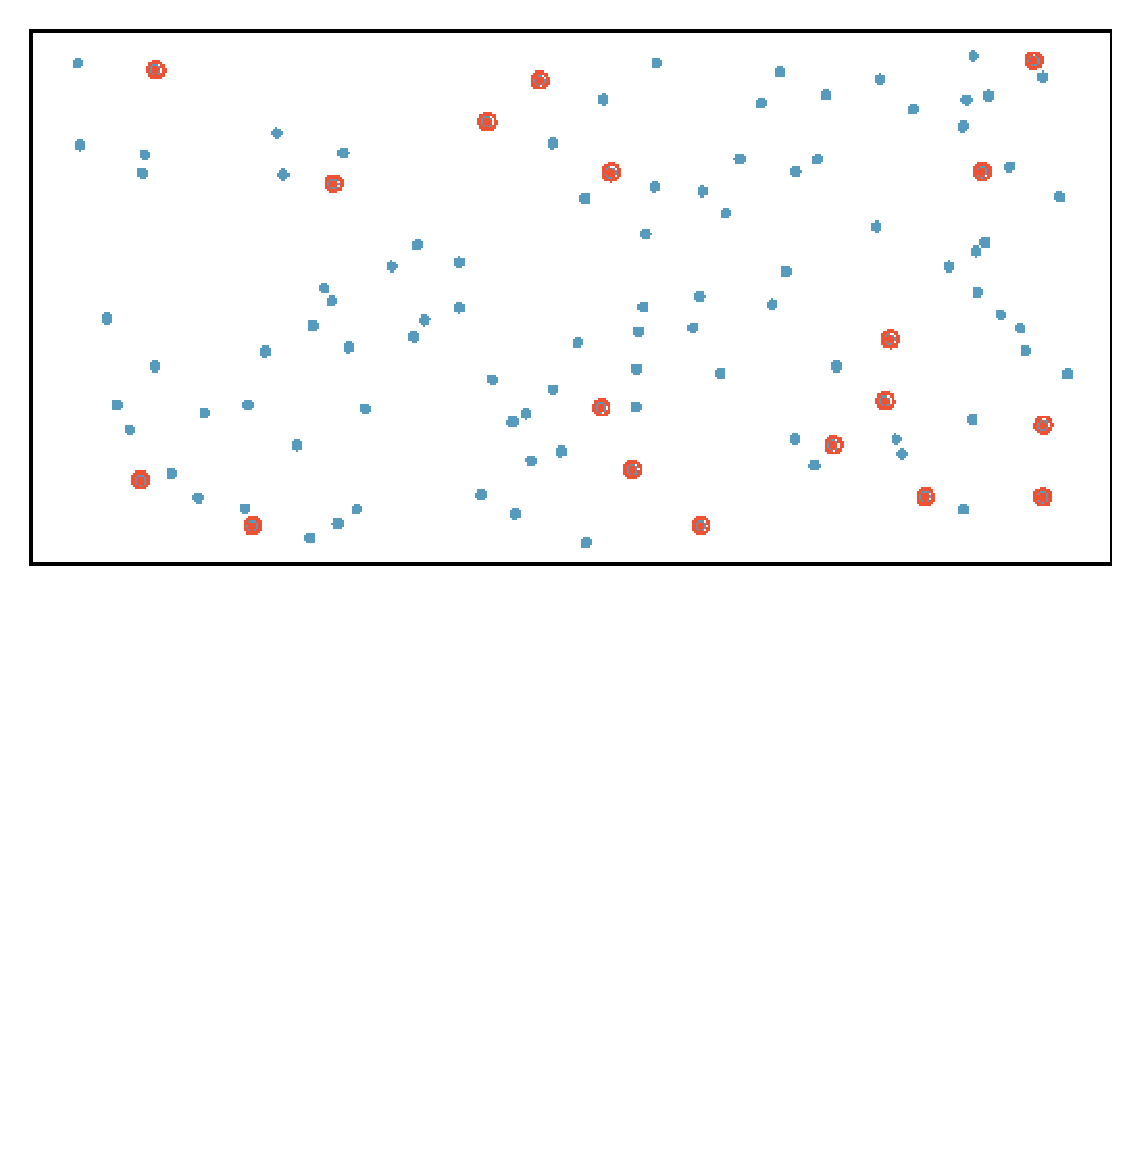
\includegraphics[width=0.9\textwidth]{1-4_obs_studies_sampling/figures/sampling_methods/simple}
\end{center}

\end{frame}

%%%%%%%%%%%%%%%%%%%%%%%%%%%%%%%%%%%%

\begin{frame}
\frametitle{Stratified sample}

\hl{Strata} are made up of similar observations. We take a simple random sample from \underline{each} stratum.

\begin{center}
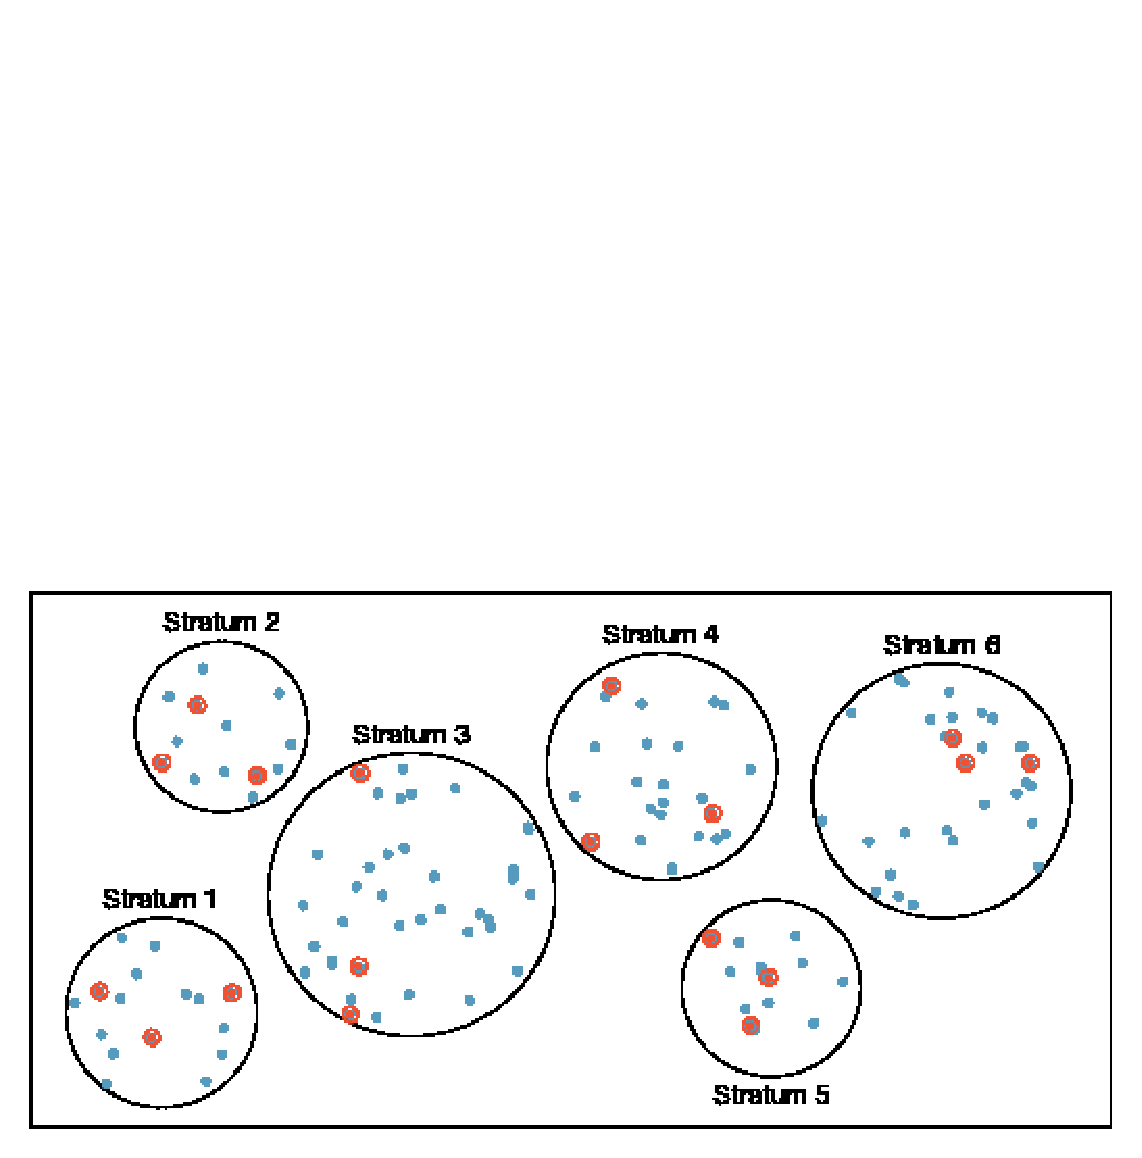
\includegraphics[width=0.9\textwidth]{1-4_obs_studies_sampling/figures/sampling_methods/stratified}
\end{center}

\end{frame}

%%%%%%%%%%%%%%%%%%%%%%%%%%%%%%%%%%%%

\begin{frame}
\frametitle{Cluster sample}

\hl{Clusters} are usually not made up of homogeneous observations. We take a simple random sample of clusters, and then sample \underline{all} observations in that cluster. Usually preferred for economical reasons.

\begin{center}
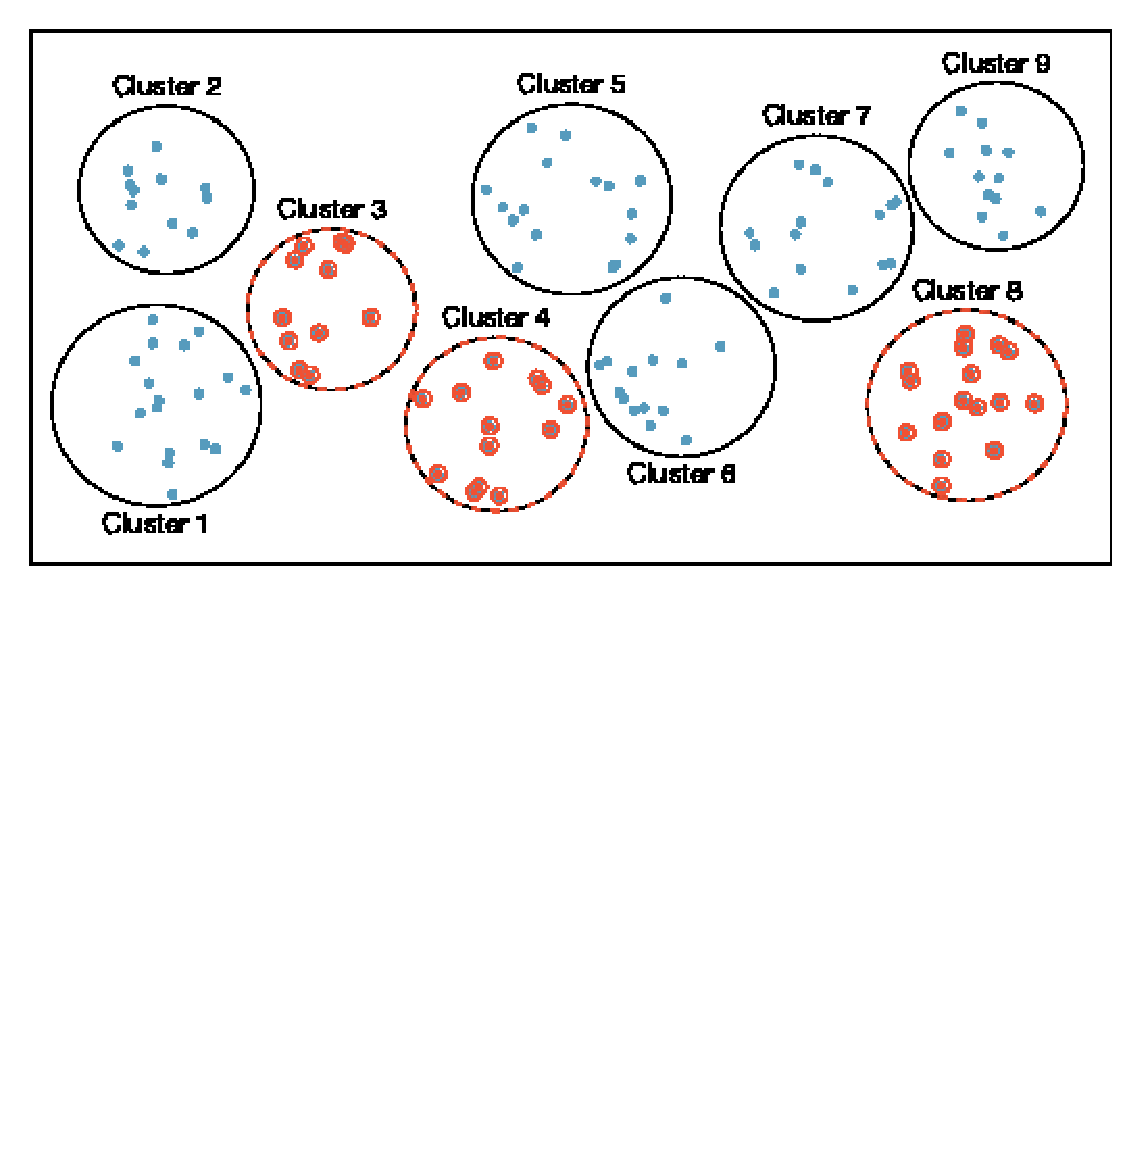
\includegraphics[width=0.9\textwidth]{1-4_obs_studies_sampling/figures/sampling_methods/cluster}
\end{center}

\end{frame}

%%%%%%%%%%%%%%%%%%%%%%%%%%%%%%%%%%%%

\begin{frame}
\frametitle{Multistage sample}

\hl{Clusters} are usually not made up of homogeneous observations.  We take a simple random sample of clusters, and then take a simple random sample of observations from the sampled clusters.

\begin{center}
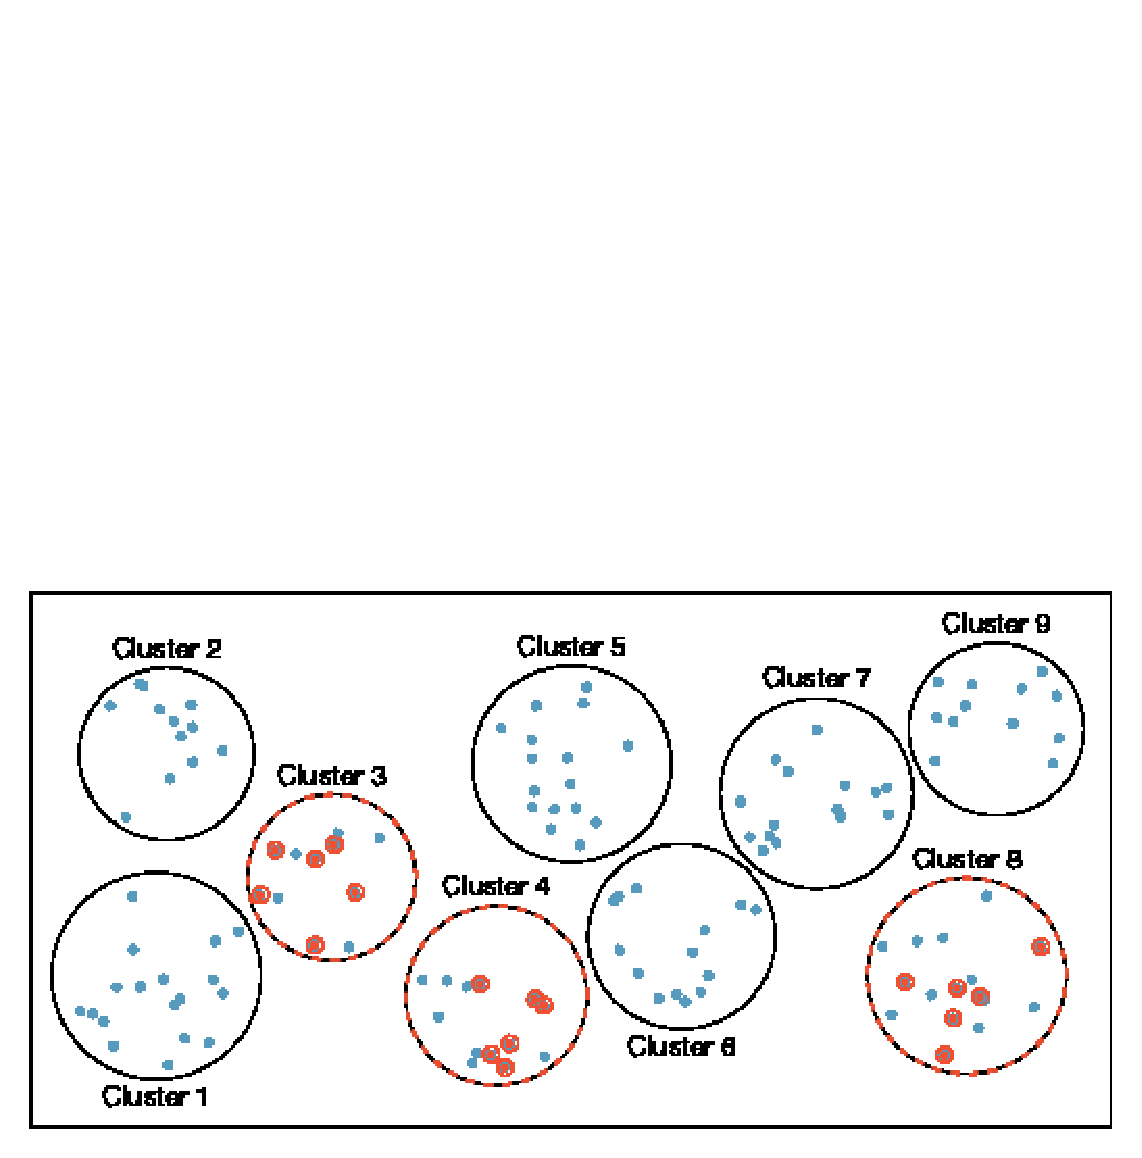
\includegraphics[width=0.9\textwidth]{1-4_obs_studies_sampling/figures/sampling_methods/multistage}
\end{center}

\end{frame}

%%%%%%%%%%%%%%%%%%%%%%%%%%%%%%%%%%%%

\begin{frame}
\frametitle{Practice}

\pq{A city council has requested a household survey be conducted in a suburban area of their city. The area is broken into many distinct and unique neighborhoods, some including large homes, some with only apartments. Which approach would likely be the \emph{least} effective?}

\begin{enumerate}[(a)]
\item Simple random sampling
\solnMult{Cluster sampling}
\item Stratified sampling
\end{enumerate}

\end{frame}

%%%%%%%%%%%%%%%%%%%%%%%%%%%%%%%%%%%%
